\documentclass[a4paper,12pt]{article}
\usepackage{../packages/coursCollege}
\newcommand{\Chapitre}{Dérivation}
\renewcommand{\path}{../../}

\renewcommand{\cours}{3MA1~--~EG~--~ns~--~2025-2026}
\usepackage{subcaption}
% Définition des couleurs
\definecolor{functioncolor}{RGB}{220,50,47}
\definecolor{tangentcolor}{RGB}{220,50,47}
\definecolor{secantcolor}{RGB}{38,139,210}
\definecolor{pointcolor}{RGB}{220,50,47}

\begin{document}

\section{La Dérivée}

\subsection{Introduction : La tangente à une courbe}

Nous commençons avec une fonction $f$, et sur le graphique nous choisissons un point $(x, f(x))$ (c.f. Figure~\ref{fig:der1}). Quelle droite, s'il y en a une, devrait être appelée tangente au graphique en ce point~? Et comment déterminer son équation~?

\begin{figure}[h]
\centering
\begin{subfigure}[c]{0.4\textwidth}
	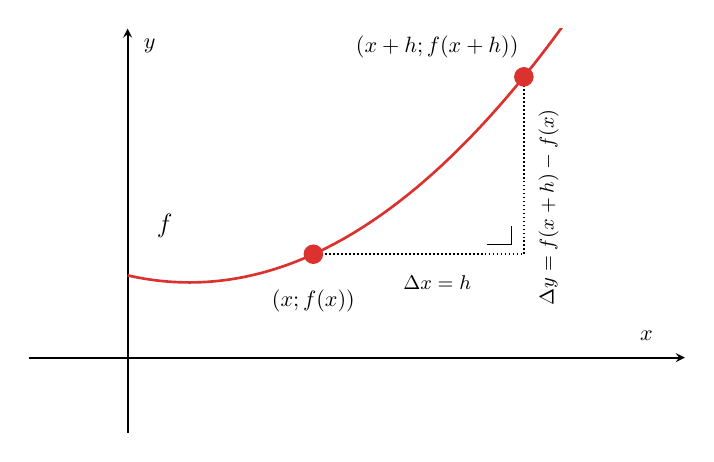
\begin{tikzpicture}[scale=0.8]
\begin{axis}[
    width=12cm,
    height=8cm,
    axis lines=middle,
    xlabel={$x$},
    ylabel={$y$},
    every axis x label/.style={at={(ticklabel* cs:0.92)}, anchor=west, yshift=10pt},
    every axis y label/.style={at={(ticklabel* cs:0.92)}, anchor=south, xshift=10pt},
    xmin=-0.8, xmax=4.5,
    ymin=-0.8, ymax=3.5,
    xtick=\empty,
    ytick=\empty,
    samples=200,
    axis line style={thick},
    every axis plot/.append style={thick},
]

% Fonction f(x) = 0.3*(x-0.5)^2 + 0.8
\addplot[
    domain=0:4,
    very thick,
    color=functioncolor,
] {0.3*(x-0.5)^2 + 0.8};

% Point (x, f(x))
\addplot[
    mark=*,
    mark size=4pt,
    color=pointcolor,
    only marks,
] coordinates {(1.5, 0.3+0.8)};
% Point (x, f(x))
\addplot[
    mark=*,
    mark size=4pt,
    color=pointcolor,
    only marks,
] coordinates {(3.2, 0.3*2.7*2.7+0.8)};

% Label du point avec fond blanc pour la lisibilité
\node[fill=white, inner sep=2pt] at (axis cs:1.5, 0.6) {$(x;f(x))$};

% Label de la fonction avec fond blanc
\node[fill=white, inner sep=2pt, font=\large] at (axis cs:0.3, 1.4) {$f$};
% Triangle de pente
% Ligne horizontale (Delta x)
\draw[thick, color=black, densely dotted] (axis cs:1.5,1.1) -- (axis cs:3.2,1.1);
% Ligne verticale (Delta y)  
\draw[thick, color=black, densely dotted] (axis cs:3.2,1.1) -- (axis cs:3.2,2.987);

% Angle droit
\draw[color=black] (axis cs:2.9,1.2) -- (axis cs:3.1,1.2) -- (axis cs:3.1,1.4);

% Labels des points
\node at (axis cs:2.5, 3.3) {$(x + h; f(x + h))$};

% Labels du triangle
\node[font=\small] at (axis cs:2.5, 0.8) {{$\Delta x = h$}};
\node[rotate=90, font=\small] at (axis cs:3.4, 1.6) {{$\Delta y = f(x+h) - f(x)$}};
\end{axis}
\end{tikzpicture}
\subcaption{Un point sur le graphe de $f$}
\end{subfigure}
\hfill
\begin{subfigure}[c]{0.48\textwidth}
	\centering
	\qrcode[height=3cm]{https://derivee.gemaths.net}
	\subcaption{Une appliquette pour visualiser différentes situations}
\end{subfigure}
\caption{Introduction à notion de dérivée}
\label{fig:der1}
\end{figure}

Pour répondre à cette question, nous choisissons un petit nombre $h \neq 0$ et sur le graphique marquons le point $(x + h, f(x + h))$. Maintenant nous traçons la droite sécante qui passe par ces deux points. La situation est illustrée dans la Figure~3.1.2 en prenant des valeurs de $h>0$.

\begin{figure}[h]
\centering
\begin{subfigure}[b]{0.4\textwidth}
\centering
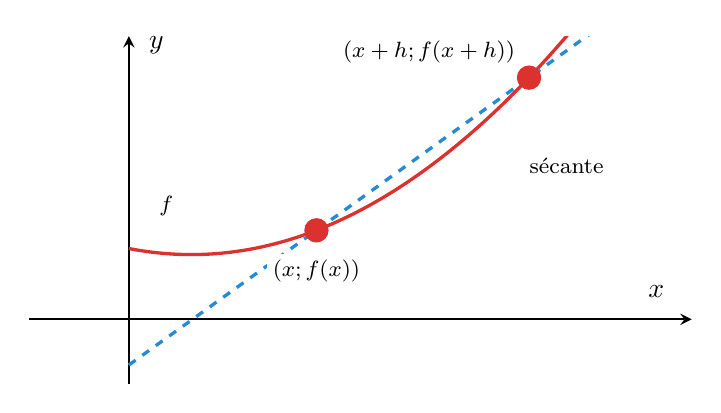
\begin{tikzpicture}
\begin{axis}[
    width=10cm,
    height=6cm,
    axis lines=middle,
    xlabel={$x$},
    ylabel={$y$},
    every axis x label/.style={at={(ticklabel* cs:0.92)}, anchor=west, yshift=10pt},
    every axis y label/.style={at={(ticklabel* cs:0.92)}, anchor=south, xshift=10pt},
    xmin=-0.8, xmax=4.5,
    ymin=-0.8, ymax=3.5,
    xtick=\empty,
    ytick=\empty,
    samples=200,
    axis line style={thick},
    every axis plot/.append style={thick},
]

% Fonction f(x) = 0.3*(x-0.5)^2 + 0.8
\addplot[
    domain=0:4,
    very thick,
    color=functioncolor,
] {0.3*(x-0.5)^2 + 0.8};

% Fonction f(x) = 0.3*(x-0.5)^2 + 0.8
\addplot[
    domain=0:4,
    very thick,
    color=secantcolor,
    dashed
] {1.11*x - 0.565};

% Point (x, f(x))
\addplot[
    mark=*,
    mark size=4pt,
    color=pointcolor,
    only marks,
] coordinates {(1.5, 0.3+0.8)};

% Point (x, f(x))
\addplot[
    mark=*,
    mark size=4pt,
    color=pointcolor,
    only marks,
] coordinates {(3.2, 0.3*2.7*2.7+0.8)};

% Label du point avec fond blanc pour la lisibilité
\node[fill=white, inner sep=2pt, font=\footnotesize] at (axis cs:1.5, 0.6) {$(x;f(x))$};
\node[fill=white, inner sep=2pt, font=\footnotesize] at (axis cs:2.4, 3.3) {$(x+h;f(x+h))$};

% Label de la fonction avec fond blanc
\node[fill=white, inner sep=2pt, font=\footnotesize] at (axis cs:0.3, 1.4) {$f$};
\node[fill=white, inner sep=2pt, font=\footnotesize] at (axis cs:3.5, 1.9) {sécante};

\end{axis}
\end{tikzpicture}
\subcaption*{$h=0,4$}
\end{subfigure}
\hfill
\begin{subfigure}[b]{0.4\textwidth}
\centering
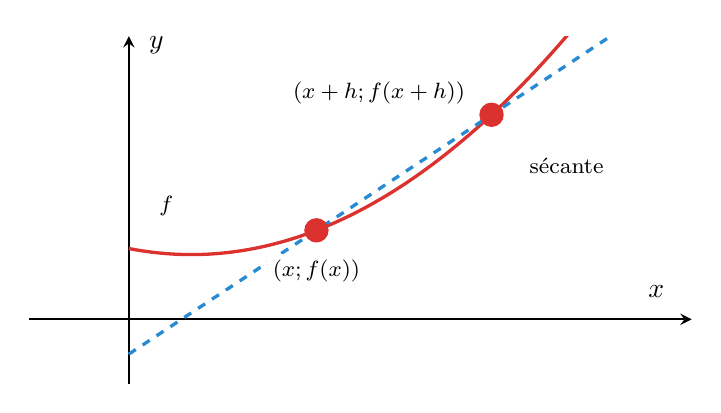
\begin{tikzpicture}
\begin{axis}[
    width=10cm,
    height=6cm,
    axis lines=middle,
    xlabel={$x$},
    ylabel={$y$},
    every axis x label/.style={at={(ticklabel* cs:0.92)}, anchor=west, yshift=10pt},
    every axis y label/.style={at={(ticklabel* cs:0.92)}, anchor=south, xshift=10pt},
    xmin=-0.8, xmax=4.5,
    ymin=-0.8, ymax=3.5,
    xtick=\empty,
    ytick=\empty,
    samples=200,
    axis line style={thick},
    every axis plot/.append style={thick},
]

% Fonction f(x) = 0.3*(x-0.5)^2 + 0.8
\addplot[
    domain=0:4,
    very thick,
    color=functioncolor,
] {0.3*(x-0.5)^2 + 0.8};

% Fonction f(x) = 0.3*(x-0.5)^2 + 0.8
\addplot[
    domain=0:4,
    very thick,
    color=secantcolor,
    dashed
] {1.02*x - 0.43};

% Point (x, f(x))
\addplot[
    mark=*,
    mark size=4pt,
    color=pointcolor,
    only marks,
] coordinates {(1.5, 0.3+0.8)};

% Point (x, f(x))
\addplot[
    mark=*,
    mark size=4pt,
    color=pointcolor,
    only marks,
] coordinates {(2.9, 0.3*2.4*2.4+0.8)};

% Label du point avec fond blanc pour la lisibilité
\node[fill=white, inner sep=2pt, font=\footnotesize] at (axis cs:1.5, 0.6) {$(x;f(x))$};
\node[fill=white, inner sep=2pt, font=\footnotesize] at (axis cs:2, 2.8) {$(x+h;f(x+h))$};

% Label de la fonction avec fond blanc
\node[fill=white, inner sep=2pt, font=\footnotesize] at (axis cs:0.3, 1.4) {$f$};
\node[fill=white, inner sep=2pt, font=\footnotesize] at (axis cs:3.5, 1.9) {sécante};

\end{axis}
\end{tikzpicture}
\subcaption*{$h=0,3$}
\end{subfigure}

\centering
\begin{subfigure}[b]{0.4\textwidth}
\centering
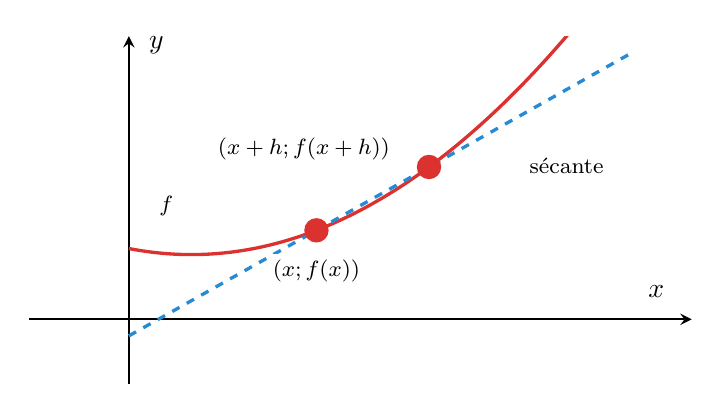
\begin{tikzpicture}
\begin{axis}[
    width=10cm,
    height=6cm,
    axis lines=middle,
    xlabel={$x$},
    ylabel={$y$},
    every axis x label/.style={at={(ticklabel* cs:0.92)}, anchor=west, yshift=10pt},
    every axis y label/.style={at={(ticklabel* cs:0.92)}, anchor=south, xshift=10pt},
    xmin=-0.8, xmax=4.5,
    ymin=-0.8, ymax=3.5,
    xtick=\empty,
    ytick=\empty,
    samples=200,
    axis line style={thick},
    every axis plot/.append style={thick},
]

% Fonction f(x) = 0.3*(x-0.5)^2 + 0.8
\addplot[
    domain=0:4,
    very thick,
    color=functioncolor,
] {0.3*(x-0.5)^2 + 0.8};

% Fonction f(x) = 0.3*(x-0.5)^2 + 0.8
\addplot[
    domain=0:4,
    very thick,
    color=secantcolor,
    dashed
] {0.87*x-0.205};

% Point (x, f(x))
\addplot[
    mark=*,
    mark size=4pt,
    color=pointcolor,
    only marks,
] coordinates {(1.5, 0.3+0.8)};

% Point (x, f(x))
\addplot[
    mark=*,
    mark size=4pt,
    color=pointcolor,
    only marks,
] coordinates {(2.4, 0.3*1.9*1.9+0.8)};

% Label du point avec fond blanc pour la lisibilité
\node[fill=white, inner sep=2pt, font=\footnotesize] at (axis cs:1.5, 0.6) {$(x;f(x))$};
\node[fill=white, inner sep=2pt, font=\footnotesize] at (axis cs:1.4, 2.1) {$(x+h;f(x+h))$};

% Label de la fonction avec fond blanc
\node[fill=white, inner sep=2pt, font=\footnotesize] at (axis cs:0.3, 1.4) {$f$};
\node[fill=white, inner sep=2pt, font=\footnotesize] at (axis cs:3.5, 1.9) {sécante};

\end{axis}
\end{tikzpicture}
\subcaption*{$h=0,15$}
\end{subfigure}
\hfill
\begin{subfigure}[b]{0.4\textwidth}
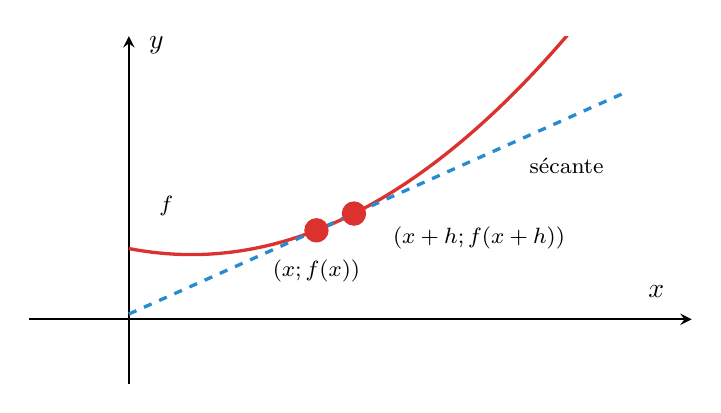
\begin{tikzpicture}
\begin{axis}[
    width=10cm,
    height=6cm,
    axis lines=middle,
    xlabel={$x$},
    ylabel={$y$},
    every axis x label/.style={at={(ticklabel* cs:0.92)}, anchor=west, yshift=10pt},
    every axis y label/.style={at={(ticklabel* cs:0.92)}, anchor=south, xshift=10pt},
    xmin=-0.8, xmax=4.5,
    ymin=-0.8, ymax=3.5,
    xtick=\empty,
    ytick=\empty,
    samples=200,
    axis line style={thick},
    every axis plot/.append style={thick},
]

% Fonction f(x) = 0.3*(x-0.5)^2 + 0.8
\addplot[
    domain=0:4,
    very thick,
    color=functioncolor,
] {0.3*(x-0.5)^2 + 0.8};

% Fonction f(x) = 0.3*(x-0.5)^2 + 0.8
\addplot[
    domain=0:4,
    very thick,
    color=secantcolor,
    dashed
] {0.69*x+0.065};

% Point (x, f(x))
\addplot[
    mark=*,
    mark size=4pt,
    color=pointcolor,
    only marks,
] coordinates {(1.5, 0.3+0.8)};

% Point (x, f(x))
\addplot[
    mark=*,
    mark size=4pt,
    color=pointcolor,
    only marks,
] coordinates {(1.8, 0.3*1.3*1.3+0.8)};

% Label du point avec fond blanc pour la lisibilité
\node[fill=white, inner sep=2pt, font=\footnotesize] at (axis cs:1.5, 0.6) {$(x;f(x))$};
\node[fill=white, inner sep=2pt, font=\footnotesize] at (axis cs:2.8, 1) {$(x+h;f(x+h))$};

% Label de la fonction avec fond blanc
\node[fill=white, inner sep=2pt, font=\footnotesize] at (axis cs:0.3, 1.4) {$f$};
\node[fill=white, inner sep=2pt, font=\footnotesize] at (axis cs:3.5, 1.9) {sécante};

\end{axis}
\end{tikzpicture}
\subcaption*{$h=0,05$}
\end{subfigure}
\caption{Construction de la dérivée}
\end{figure}
\hfill

\vspace{0.5cm}

Lorsque $h$ tend vers zéro (une limite!), la droite sécante tend (si la limite existe) vers « la tangente de $f$ au point $(x, f(x))$ ».

Puisque les droites sécantes ont une pente de la forme
\begin{equation}
\frac{f(x + h) - f(x)}{h}, \quad \text{(vérifiez ceci)}
\end{equation}

nous affirmons que la position limite de ces sécantes ont une pente
\begin{equation}
\lim_{h \to 0} \frac{f(x + h) - f(x)}{h}.
\end{equation}

\subsection*{Dérivées et Différentiation}

Dans l'introduction nous avons parlé de manière informelle des droites tangentes et avons donné une interprétation géométrique aux limites de la forme
\begin{equation}
\lim_{h \to 0} \frac{f(x + h) - f(x)}{h}.
\end{equation}

Ici nous commençons l'étude systématique de telles limites, ce que les mathématiciens appellent la théorie de la \emph{différentiation}.

\begin{center}
\rule{\textwidth}{0.4pt}
\end{center}

\textbf{Définition 3.1.1}

Une fonction $f$ est dite \emph{dérivable} (ou \emph{différentiable}) en $x$ si et seulement si
\begin{equation}
\lim_{h \to 0} \frac{f(x + h) - f(x)}{h} \quad \text{existe}.
\end{equation}

Si cette limite existe, elle est appelée la \emph{dérivée} de $f$ en $x$ et est notée $f'(x)$.

\begin{center}
\rule{\textwidth}{0.4pt}
\end{center}

Nous interprétons
\begin{equation}
f'(x) = \lim_{h \to 0} \frac{f(x + h) - f(x)}{h}
\end{equation}
comme la \emph{pente du graphique au point} $(x, f(x))$ ou, ce qui revient au même, comme la pente de la droite tangente au graphique au point $(x, f(x))$.

\newpage

% Figure supplémentaire illustrant le triangle de pente
\begin{figure}[h]
\centering
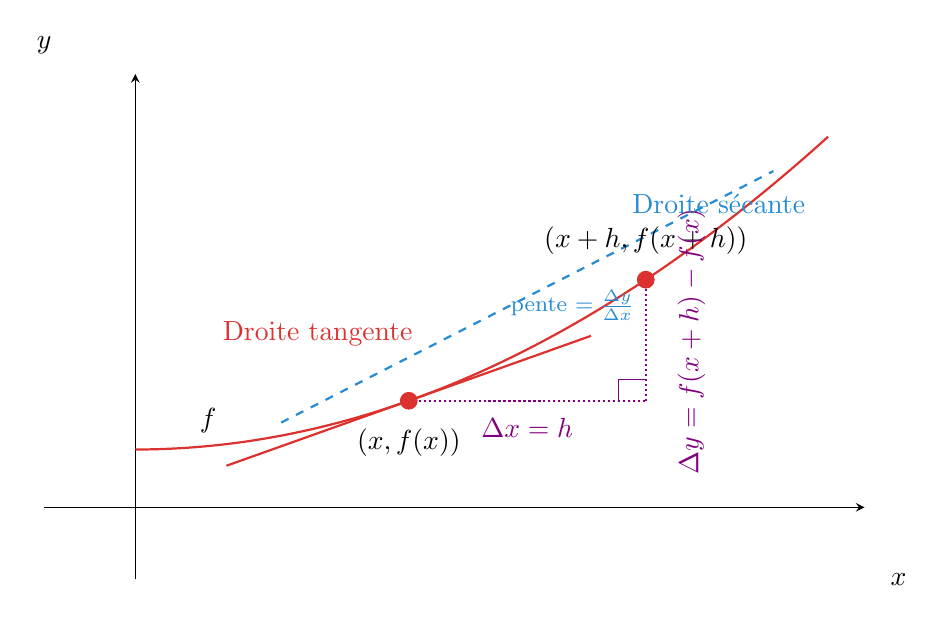
\begin{tikzpicture}
\begin{axis}[
    width=12cm,
    height=8cm,
    axis lines=middle,
    xlabel={$x$},
    ylabel={$y$},
    xlabel style={at={(axis description cs:1.02,0)}, anchor=west},
    ylabel style={at={(axis description cs:0,1.02)}, anchor=south},
    xmin=-0.5, xmax=4,
    ymin=-0.5, ymax=3,
    xtick=\empty,
    ytick=\empty,
    samples=100,
    grid=major,
    grid style={gray!20},
]

% Fonction f(x) = 0.15*x^2 + 0.4
\addplot[
    domain=0:3.8,
    thick,
    color=functioncolor,
] {0.15*x^2 + 0.4};

% Points
\addplot[
    mark=*,
    mark size=3pt,
    color=pointcolor,
    only marks,
] coordinates {(1.5, 0.7375) (2.8, 1.576)};

% Droite sécante
\addplot[
    domain=0.8:3.5,
    thick,
    color=secantcolor,
    dashed,
] {0.645*x + 0.0705};

% Droite tangente approximative au point (1.5, 0.7375)
\addplot[
    domain=0.5:2.5,
    thick,
    color=tangentcolor,
] {0.45*x + 0.0625};

% Triangle de pente
% Ligne horizontale (Delta x)
\draw[thick, color=violet, densely dotted] (axis cs:1.5,0.7375) -- (axis cs:2.8,0.7375);
% Ligne verticale (Delta y)  
\draw[thick, color=violet, densely dotted] (axis cs:2.8,0.7375) -- (axis cs:2.8,1.576);

% Angle droit
\draw[color=violet] (axis cs:2.65,0.7375) -- (axis cs:2.65,0.8875) -- (axis cs:2.8,0.8875);

% Labels des points
\node at (axis cs:1.5, 0.45) {$(x, f(x))$};
\node at (axis cs:2.8, 1.85) {$(x + h, f(x + h))$};

% Labels du triangle
\node at (axis cs:2.15, 0.55) {\textcolor{violet}{$\Delta x = h$}};
\node[rotate=90] at (axis cs:3.05, 1.15) {\textcolor{violet}{$\Delta y = f(x+h) - f(x)$}};

% Label de la pente
\node at (axis cs:2.4, 1.4) {\textcolor{secantcolor}{\footnotesize pente $= \frac{\Delta y}{\Delta x}$}};

% Label de la fonction
\node at (axis cs:0.4, 0.6) {$f$};

% Labels des droites
\node at (axis cs:3.2, 2.1) {\textcolor{secantcolor}{Droite sécante}};
\node at (axis cs:1.0, 1.2) {\textcolor{tangentcolor}{Droite tangente}};

\end{axis}
\end{tikzpicture}
\caption{Triangle de pente illustrant la définition géométrique de la dérivée}
\end{figure}

\textbf{Interprétation géométrique :}
\begin{itemize}
\item Le rapport $\frac{\Delta y}{\Delta x} = \frac{f(x+h) - f(x)}{h}$ représente la pente de la droite sécante.
\item Lorsque $h \to 0$, ce rapport tend vers $f'(x)$, la pente de la droite tangente.
\item Le triangle rectangle formé par $\Delta x$ et $\Delta y$ illustre visuellement cette notion de pente.
\end{itemize}

\textbf{Notations alternatives :}
\begin{align}
f'(x) &= \lim_{h \to 0} \frac{f(x + h) - f(x)}{h} \\
&= \lim_{\Delta x \to 0} \frac{\Delta y}{\Delta x} \\
&= \lim_{\Delta x \to 0} \frac{f(x + \Delta x) - f(x)}{\Delta x} \\
&= \frac{dy}{dx} \bigg|_{x} \quad \text{(notation de Leibniz)}
\end{align}

\end{document}
